Energi-gapet mellom valensbåndet og ledningsbåndet
kan variere for forksjellige stoffer.
Store gap, som gjør det vanskelig for et elektron å nå ledningsbåndet,
er karakteristisk for isolatorer.
Tilsvarende er gapet mindre i halvledere.
Og i ledere er det er overlapp mellom valensbåndet og ledningsbåndet,
som gjør at det leder strøm ved romtemperatur.
\\\\
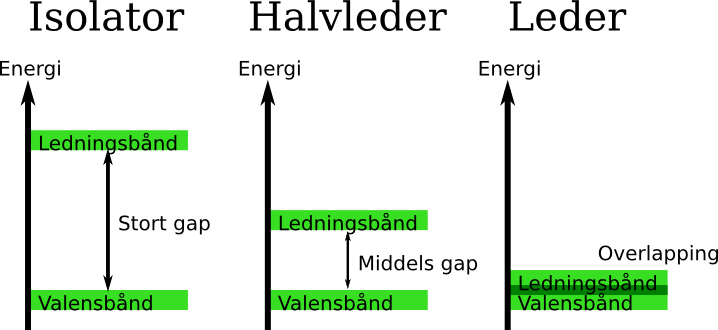
\includegraphics[width=\textwidth]{./img/energigap}
